
\subsubsection{25.10.14}

\begin{enumerate}
	\item The time of beginning and ending of the meeting:
	16:00 - 20:00
	\item Purposes of the meeting:
	\begin{enumerate}
	  \item To elaborate and create the mechanism of capture movable baskets. 
	  
    \end{enumerate}
    
	\item Work that has been done:
	\begin{enumerate}
	  \item They was considered 2 options of mechanism capture movable baskets (hereinafter it will be called MCB):
	  \begin{enumerate}
	    \item Servo with the beam. When servo rotates beam turns and lowers.
	    
	    \item The furniture slat which connected with servo by the fishing line is fixed to the rear edge of robot. When servo rotates slat lowers.
	    
	    \begin{figure}[H]
	    	\begin{minipage}[h]{0.2\linewidth}
	    		\center   
	    	\end{minipage}
	    	\begin{minipage}[h]{0.6\linewidth}
	    		\center{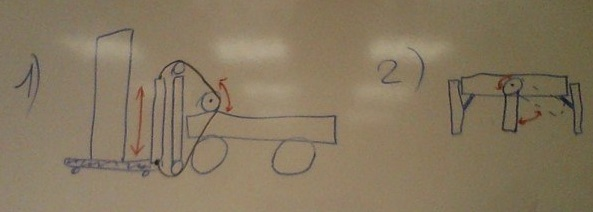
\includegraphics[scale=0.55]{days/25.10.14/images/01}}
	    		\caption{Ideas of MCB 1)Slat 2)Servo with beam}
	    	\end{minipage}
	    \end{figure}
	    
      \end{enumerate}
      \item It was decided to make MCB with slat because this variant more compact.
      
      \item The furniture slat was sawn for reduction it's length.
      
      \begin{figure}[H]
      	\begin{minipage}[h]{0.2\linewidth}
      		\center   
      	\end{minipage}
      	\begin{minipage}[h]{0.6\linewidth}
      		\center{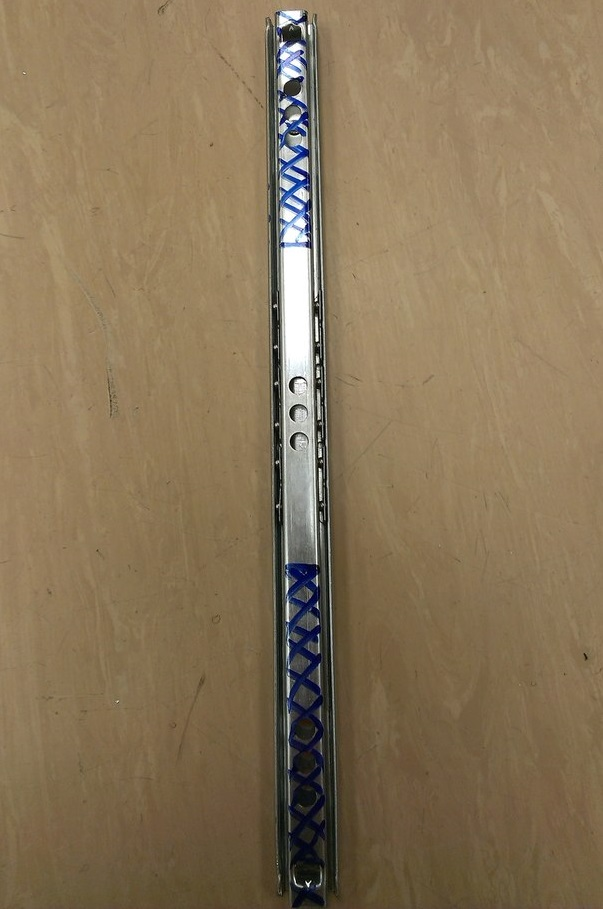
\includegraphics[scale=0.24]{days/25.10.14/images/02}}
      		\caption{Shortened furniture slat \newline (the sawn part is hatched)}
      	\end{minipage}
      \end{figure}
      
      \item They were marked location for drilling holes for mounts on the slat. The holes weren't drilled because we didn't have the drill.
      
    \end{enumerate}
    
	\item Results: 
	\begin{enumerate}
	  \item MCB was elaborated but didn't installed.
      
    \end{enumerate}
    
	\item Tasks for the next meetings:
	\begin{enumerate}
	  \item To finish creating of MCB.
	  
    \end{enumerate}     
\end{enumerate}
\fillpage
